\documentclass{beamer} % Использование класса beamer для создания презентации
\usetheme{Boadilla} % Применение темы Boadilla

\usepackage[T2A]{fontenc} % Установка кодировки шрифта
\usepackage[utf8]{inputenc} % Установка кодировки исходного текста
\usepackage[english,russian]{babel} % Подключение локализации и переносов для русского и английского языков
\usepackage{amsmath,amssymb} % Подключение математических символов и формул
\usepackage{autonum} % Автоматическая нумерация формул только при наличии ссылок на них
\usepackage{wrapfig} % Подключение пакета для обтекания текстом рисунков и таблиц
\usepackage{array} % Подключение пакета для работы с таблицами

\newcommand{\PreserveBackslash}[1]{\let\temp=\\#1\let\\=\temp} % Команда для сохранения обратной косой черты в ячейках таблицы
\newcolumntype{C}[1]{>{\PreserveBackslash\centering}p{#1}} % Создание нового типа столбца с центрированным содержимым

\usepackage[labelformat=empty]{caption} % Подключение пакета для настройки подписей и удаление названия "Рисунок"
\graphicspath{{./images/}{./images/logo/}} % Указание папок, где искать изображения

\setbeamertemplate{navigation symbols}{} % Удаление навигационных символов на слайдах
\usepackage{ragged2e} % Подключение пакета для улучшенного выравнивания текста
\newcommand{\jj}{\righthyphenmin=20 \justifying} % Команда для активации выравнивания по ширине с установкой минимального количества символов в слове перед переносом



\begin{document}




\begin{frame}
  \begin{center}\tiny
    Федеральное государственное бюджетное образовательное учреждение высшего образования \\
    «Московский государственный технический университет имени Н.Э. Баумана (национальный исследовательский университет)» (МГТУ им. Н.Э. Баумана)\\
    Факультет «Фундаментальные науки»\\
    Кафедра «Физика»
  \end{center}

  \begin{center}
    
\includegraphics[width=0.15\linewidth]{emb}
  \end{center}

  \begin{center}\tiny
    \textbf{КВАЛИФИКАЦИОННАЯ РАБОТА МАГИСТРА ТЕХНИКА И ТЕХНОЛОГИИ \\ ПО НАПРАВЛЕНИЮ 14040000.62 «ТЕХНИЧЕСКАЯ ФИЗИКА»}\\
    \vspace{0.2cm}
    \textbf{НА ТЕМУ:}\\
    \vspace{0.1cm}
    \textbf{<<РОЛЬ ДАЛЬНОДЕЙСТВИЯ ПРИТЯЖЕНИЯ В \\ ДИФФУЗИИ И СПЕКТРАХ ВОЗБУЖДЕНИЙ ПРОСТЫХ ЖИДКОСТЕЙ>>}
  \end{center}

  \vspace{0.3cm}

  \begin{columns}
    \begin{column}{0.50\textwidth}
      \begin{center}\tiny
        Выполнил: \\
        \vspace{0.1cm}
        \textbf{Дмитрюк Никита Александрович}\\
        студент группы ФН4-41M \\
      \end{center}
    \end{column}

    \begin{column}{0.50\textwidth}
      \begin{center}\tiny
        Научный руководитель:\\
        \vspace{0.1cm}
        \textbf{Юрченко Станислав Олегович} \\
        д.ф.-м.н., профессор кафедры физики\\
        МГТУ им. Н.Э. Баумана \\
      \end{center}
    \end{column}
  \end{columns}

  \vspace{0.5cm}
  \begin{center}\tiny
    Москва, $2022$
  \end{center}
\end{frame}




\begin{frame}{Актуальность}
  \footnotesize{

    \textbf{Актуальность:}

    Остаются открытыми такие важные вопросы, как влияние потенциала взаимодействия между частицами на температурную зависимость коэффициента диффузии и насколько важны корреляции между спектрами возбуждения частиц и транспортными свойствами, а также, какую роль играет дальнодействие притяжения в скорости нуклеации в переохлажденных системах

    \vspace{1cm}

    \textbf{Практическая значимость:}

    \begin{itemize}
    \item Численно рассчитана диффузия и спектры на жидкостной бинодали веществ
    \item Разработан новый метод распознавания фаз, который универсален по отношению к размерности системы и формам кластеров, с сохранением точности расчета на уровне других методов
    \end{itemize}
  }
\end{frame}




\begin{frame}{Цель и задачи работы}
  \footnotesize{

    \textbf{Цель работы} -- установить связь дальнодействия притяжения потенциала взаимодействия и спектров возбуждений с транспортными свойствами жидкостей, а также выявить влияние дальнодействия притяжения на скорость нуклеации.

    \vspace{0.5cm}

    \textbf{Задачами работы являются:}
    \begin{itemize}
    \item Расчет фазовых диаграмм для 2D и 3D систем частиц, взаимодействующих посредством обобщенного потенциала Леннарда-Джонса с различными степенями притяжения.
    \item Адаптация метода кластеризации данных DBSCAN для изучения молекулярных систем и его сравнение с другими методами.
    \item Расчет и анализ транспортных свойств и коллективных возбуждений на жидкостных бинодалях.
    \item Применение нового метода распознавания фаз для изучения скорости нуклеации в переохлажденных системах Леннарда-Джонса с различным дальнодействием притяжения.
    \end{itemize}
  }
\end{frame}




\begin{frame}{Положения, выносимые на защиту}
  \footnotesize{

    \begin{enumerate}
    \item Температурная зависимость диффузии имеет линейную зависимость в широком диапазоне температур на бинодали жидкость-газ, отклонение от которой коррелирует с изменением характера спектра возбуждений. Отношение температур критической к тройной точке убывает с уменьшением дальнодействия потенциала взаимодействия
    \item Разработанный метод распознавания фаз на основе алгоритма кластеризации обладает универсальностью как к размерности системы так и к форме кластеров с сохранением точности на уровне других методов
    \end{enumerate}
  }
\end{frame}




\begin{frame}{Метод молекулярной динамики}
  \footnotesize{

    \begin{columns}
      \begin{column}{0.4\linewidth}

        \centering
        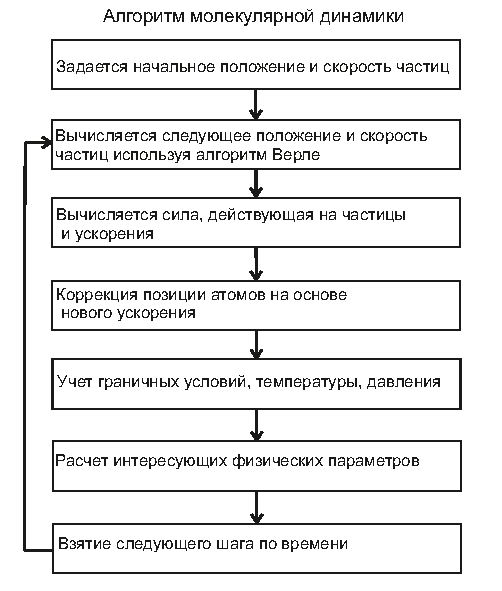
\includegraphics[width=\textwidth]{blocksheme}

      \end{column}

      \begin{column}{0.5\linewidth}

        \begin{figure}
          \centering
          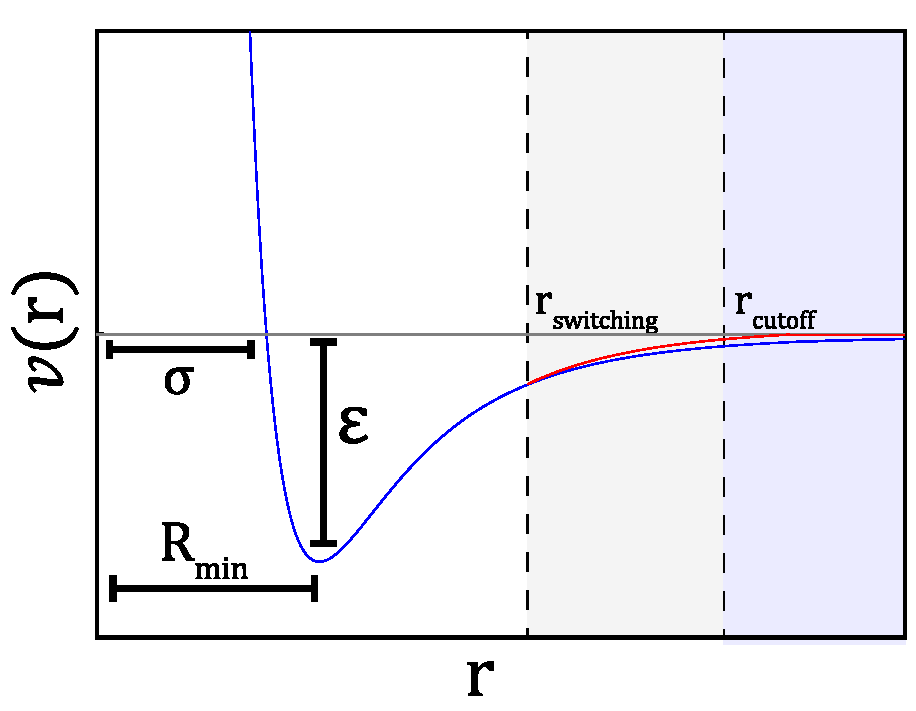
\includegraphics[width=\textwidth]{Lj-cutoff-scheme}
        \end{figure}

      \end{column}
    \end{columns}

    \centering \textbf{Алгоритм Верле:}

    \begin{equation}
      \overrightarrow{\mathrm{r}}(\mathrm{t}+\Delta \mathrm{t})=2 \overrightarrow{\mathrm{r}}(\mathrm{t})-\overrightarrow{\mathrm{r}}(\mathrm{t}-\Delta \mathrm{t})+\overrightarrow{\mathrm{a}}(\mathrm{t}) \Delta \mathrm{t}^{2}+\mathrm{O}\left(\Delta \mathrm{t}^{4}\right), \hspace{0.1cm} \text{где} \hspace{0.2cm} \vec{a}(t)=-\frac{\operatorname{grad}(\mathrm{U}(\mathrm{\overrightarrow{r}}(\mathrm{t})))}{\mathrm{m}}
    \end{equation}
  }
\end{frame}




\begin{frame}{Параметры моделирований}
  \footnotesize{

    \begin{columns}
      \begin{column}{0.5\linewidth}

        \centering \textbf{LJn-m}

        \begin{equation}
          U_{n-m}(r)=4 \varepsilon\left[\left(\frac{\sigma}{r}\right)^{n}-\left(\frac{\sigma}{r}\right)^{m}\right]
          \label{eqGenLJ}
        \end{equation}
        \jj где $\epsilon = 1$ и $\sigma = 1$ - магнитуда и \\ характерный масштаб отталкивания соответственно.

        \vspace{0.0cm}

        \begin{figure}
          \centering
          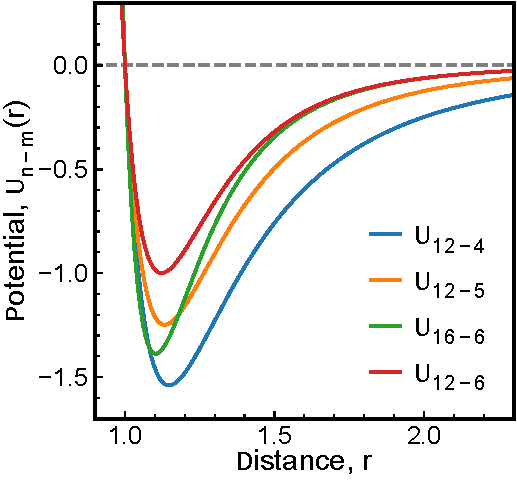
\includegraphics[width=0.8\textwidth]{LJ_no_norm.pdf}
        \end{figure}

      \end{column}

      \begin{column}{0.5\linewidth}

        \vspace{0.4cm}
        \centering \textbf{Ethane}

        \begin{equation}
          U_{ethane}(r) = \tilde \varepsilon\left[\left(\frac{\sigma}{r}\right)^{16}-\left(\frac{\sigma}{r}\right)^{6}\right],
          \label{eqEthan}
        \end{equation}
        \jj где $\tilde \varepsilon = 0.695$ ккал/моль; $\sigma = 3.783$\AA.

        \vspace{1.0cm}

        \begin{figure}
          \centering
          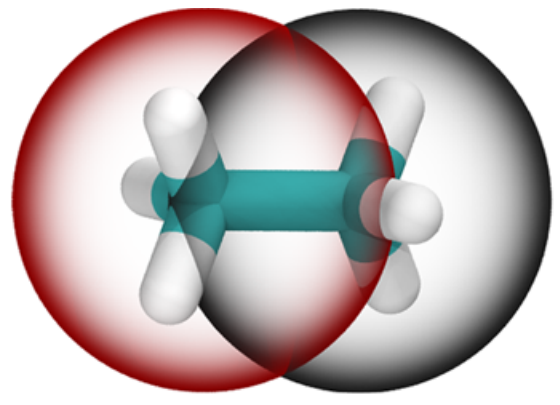
\includegraphics[width=0.7\textwidth]{ethane2.png}
        \end{figure}

        \vspace{0.5cm}

      \end{column}
    \end{columns}
  }

  \tiny{J. R. Mick, et al., Journal of Chemical $\And$ Engineering Data 62, 1806 (2017).}

\end{frame}




\begin{frame}{Построение фазовых диаграмм}
  \footnotesize{

    \begin{columns}
      \begin{column}{0.55\linewidth}

        \vspace{0.5cm}
        \begin{figure}
          \centering
          \href{run:video_flat_layer.mp4}{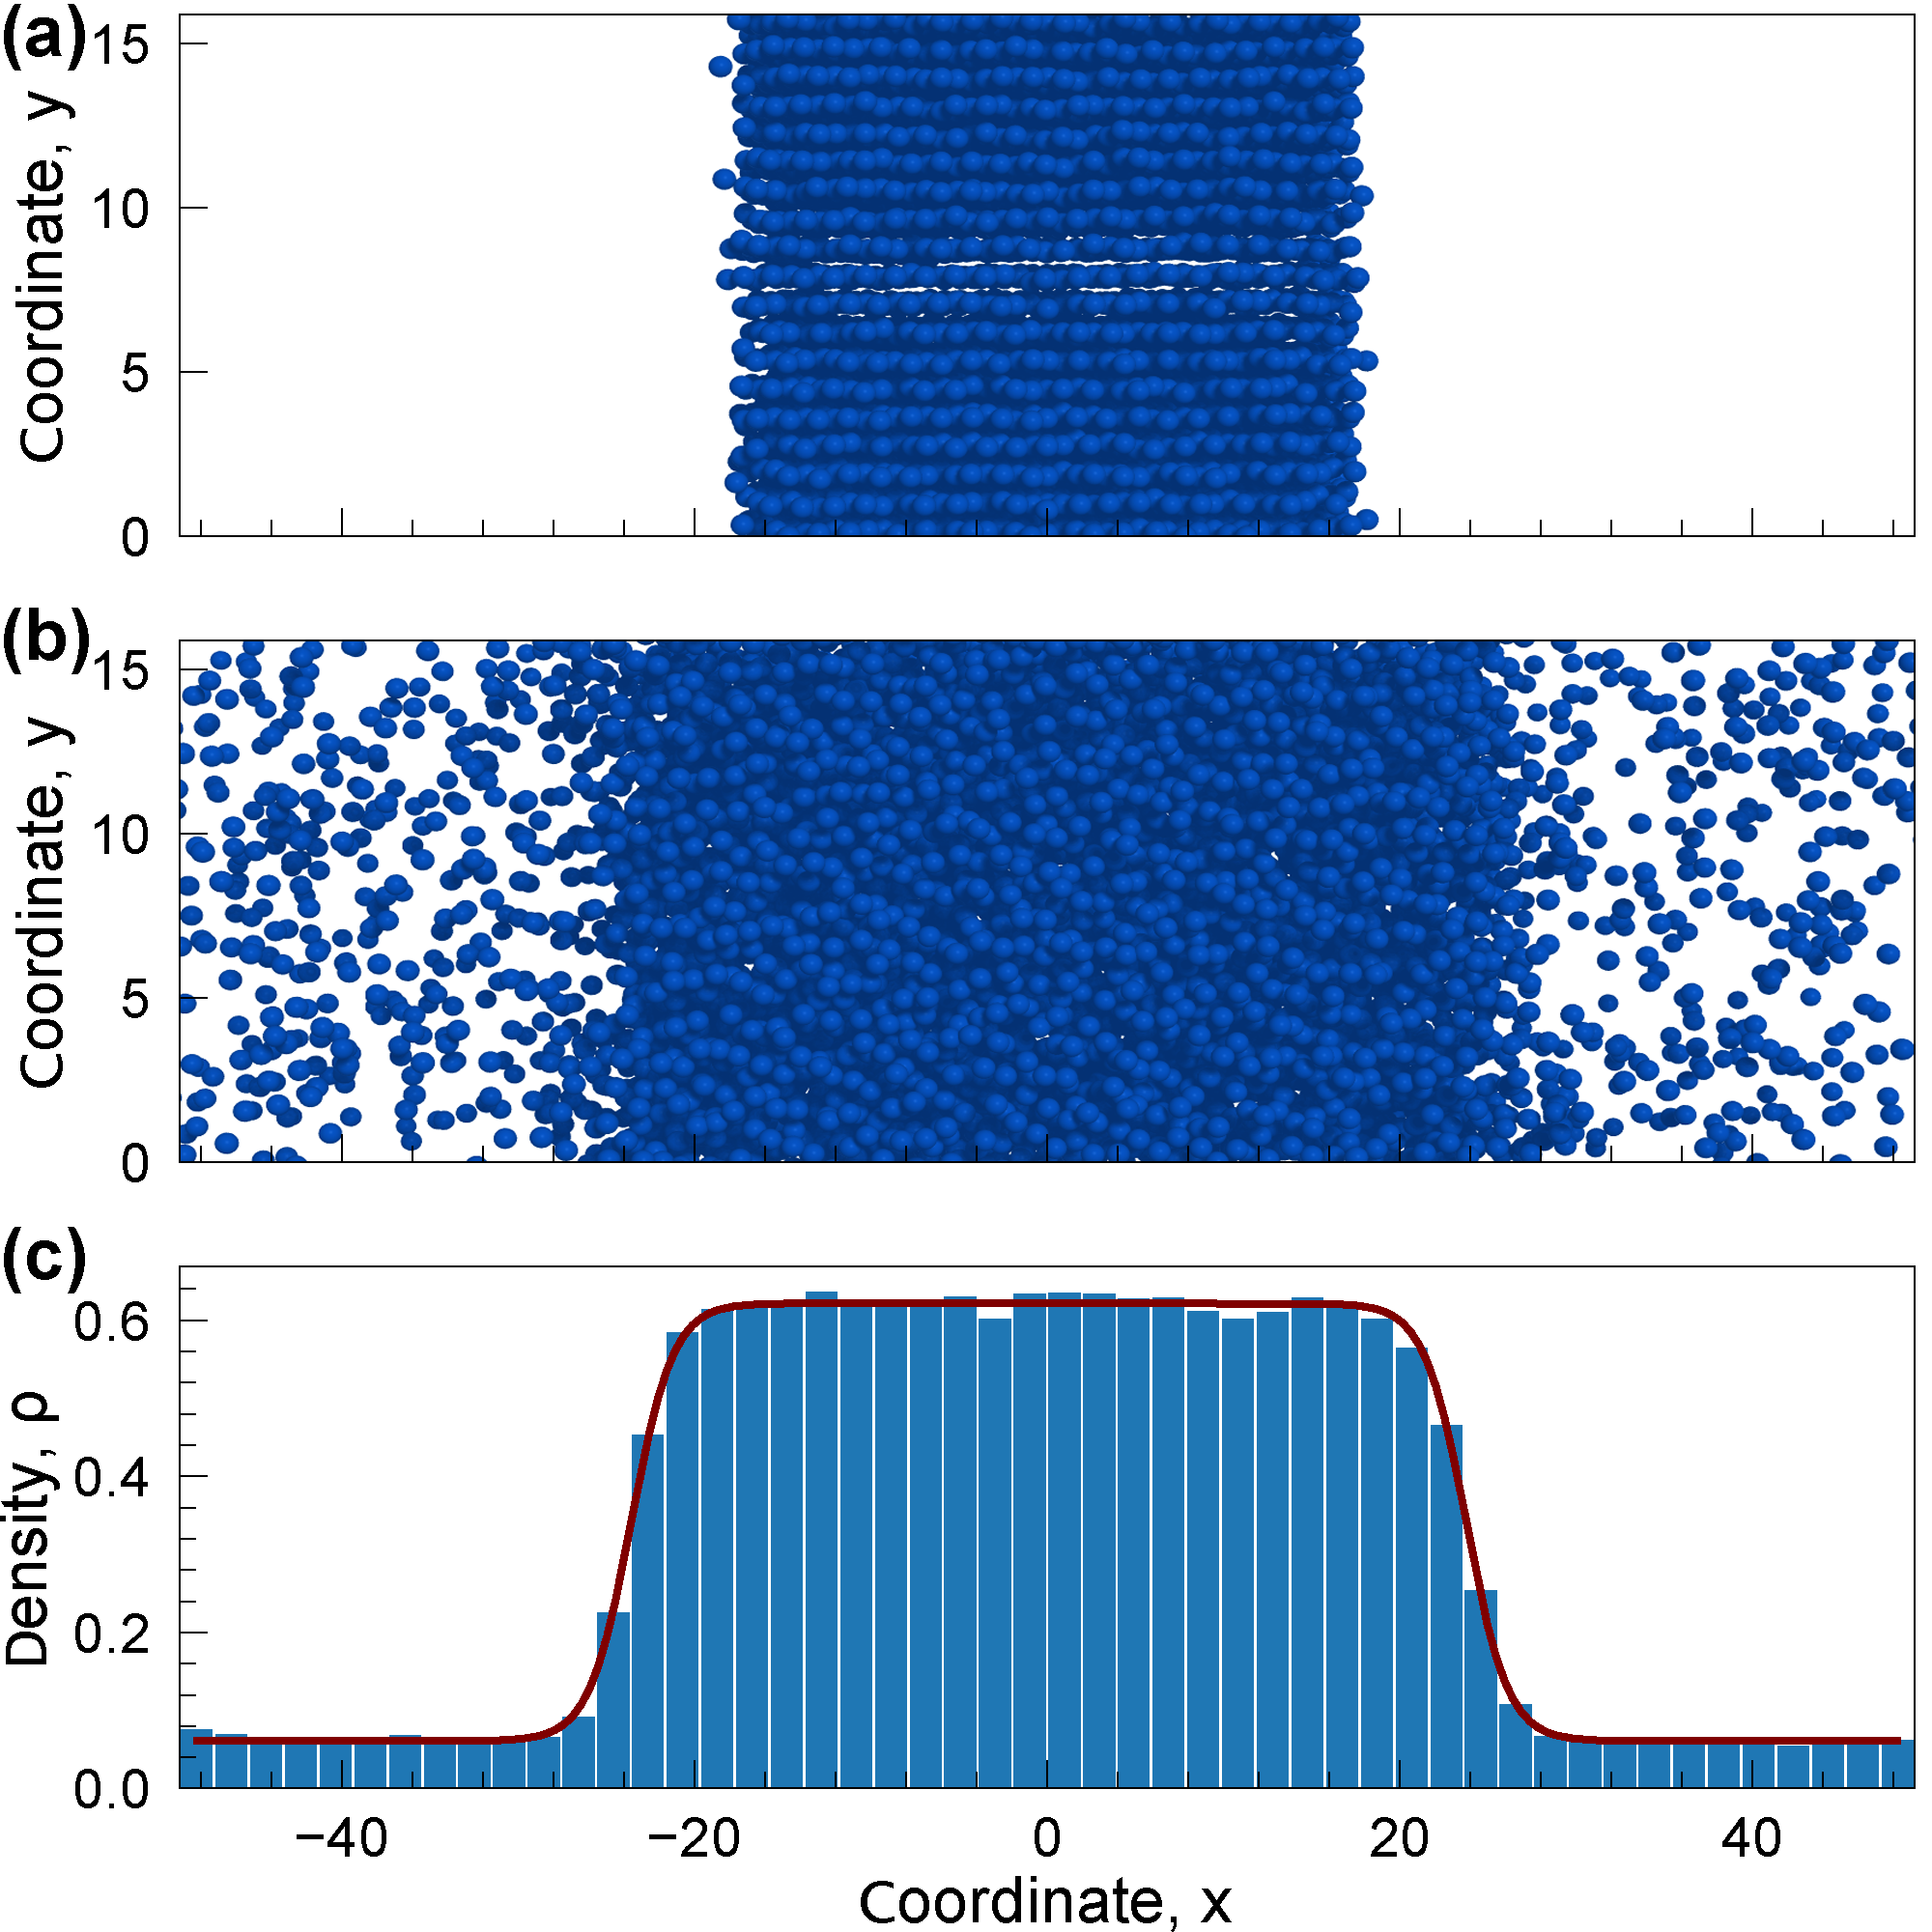
\includegraphics[width=\textwidth]{MACR-Figure0.png}}

        \end{figure}

      \end{column}

      \begin{column}{0.48\linewidth}

        \begin{equation}
          \rho(x)=\frac{\rho_{c}+\rho_{g}}{2}-\frac{\rho_{c}-\rho_{g}}{2} \tanh \left(\frac{|x|-L}{\delta}\right)
        \end{equation}
        \jj{где $L$ - половина размера области \\ конденсированной фазы; \\
          $\delta$ - характерная толщина
          интерфейса.}

        \vspace{0.5cm}

        \begin{table}[h!]
          \footnotesize
          \centering
          \begin{tabular}{c|c|c|c|c}
            LJ$n$-$m$ & $\rho$ & $r_c$ & $T_{\rm start}$ & $T_{\rm stop}$ \\ \hline
            LJ12-4 & 0.25 & 15.0 & 1.0 & 5.5 \\
            LJ12-5 & 0.25 & 10.0 & 0.8 & 2.4\\
            LJ12-6 & 0.35 & 8.0 & 0.5 & 1.4\\
            LJ16-6 & 0.31 & 8.0 & 0.8 & 1.6\\
          \end{tabular}

          \label{MACR-Table1}
        \end{table}

      \end{column}
      \begin{column}{0.001\linewidth}
      \end{column}
    \end{columns}
  }

  \vspace{0.5cm}
  \tiny{F. Biscay, et al., The Journal of Physical Chemistry B 112, 13885 (2008).}

\end{frame}




\begin{frame}{Принцип работы DBSCAN}
  \footnotesize{

    \begin{figure}[!t]
      \centering
      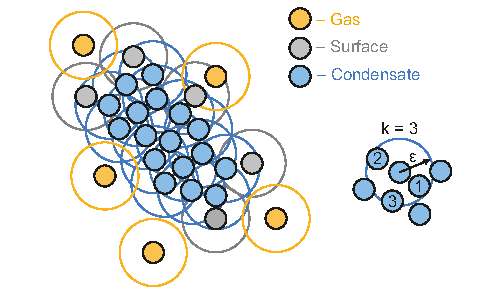
\includegraphics[width=0.9\linewidth]{kepsilon.pdf}
      \caption{Принцип работы алгоритма кластеризации DBSCAN для случая $k = 3$.}
      \label{kepsilon}
    \end{figure}
  }

\end{frame}




\begin{frame}{Пример распознавания частиц в 2D системе LJ12-6.}
  \footnotesize{

    \begin{figure}[!t]
      \centering
      \includegraphics[width=0.8\linewidth]{PRIMe-FIgure104.pdf}
      \caption{(a) классификация частиц на конденсат и газ. \\
        (b) выделение частиц поверхности, по условию принадлежности к конденсату и не к основным частицам. \\
        (с) пример выделения регулярной поверхности, охватывающей все частицы кластера.}
      \label{DBSCAN-Illustr}
    \end{figure}
  }
\end{frame}




\begin{frame}{Распознавание фаз методом DBSCAN в 3D системе LJ12-6}
  \footnotesize{
    \begin{figure}[!t]
      \centering
      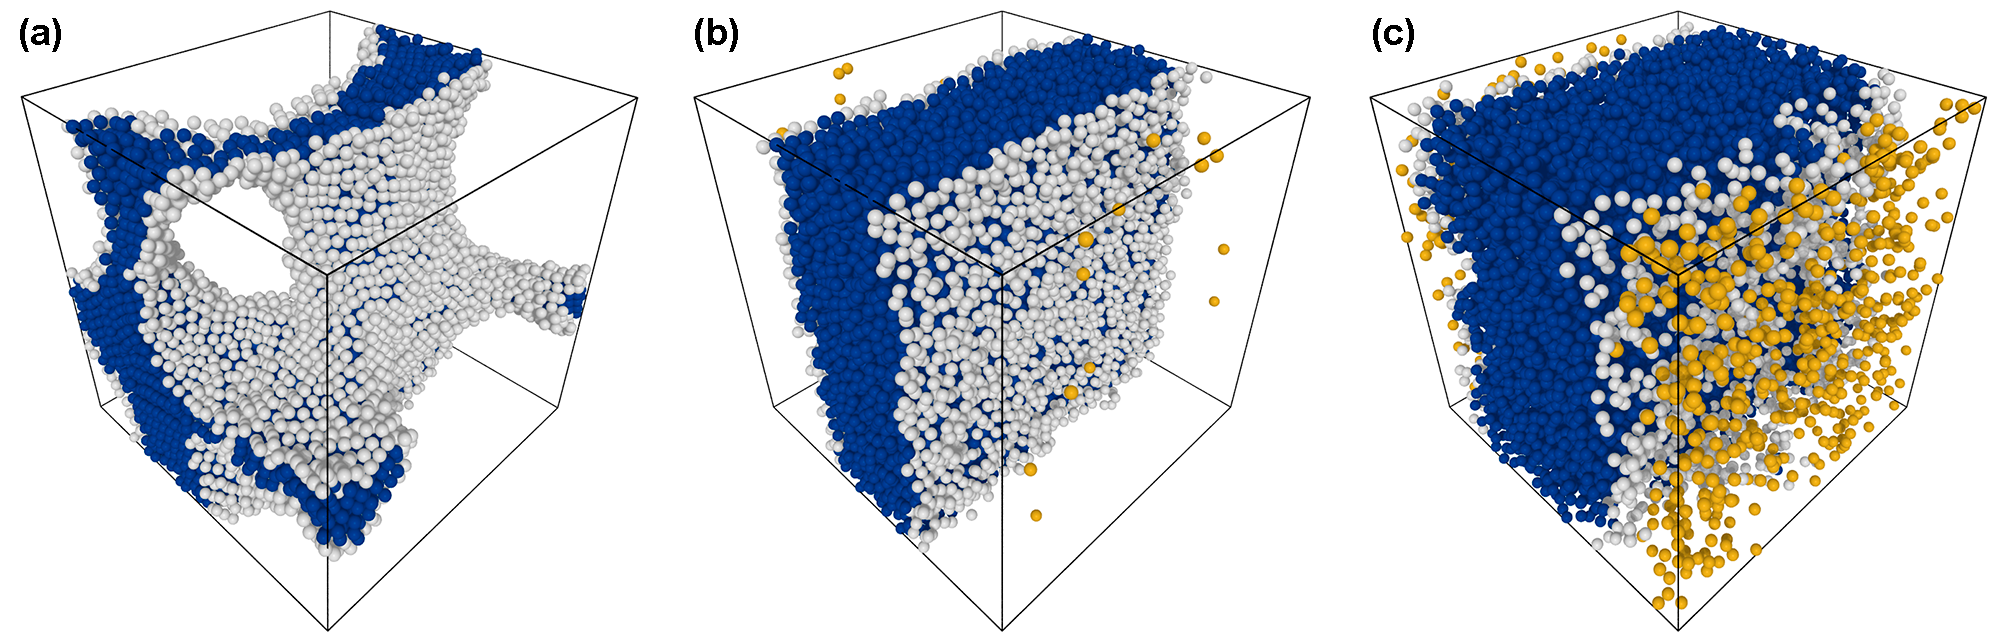
\includegraphics[width=\linewidth]{PRIMe-Figure103.png}
      \caption{(a) кластер произвольной формы при температуре ниже тройной точки. \\
        (b) система в состоянии жидкость + газ. \\
        (с) система вблизи критической точки.}
      \label{D3_free_conf}
    \end{figure}
  }
\end{frame}




\begin{frame}{Нахождение критических точек}
  \footnotesize{
    \begin{columns}
      \begin{column}{0.6\linewidth}

        \vspace{0.1cm}

        \begin{figure}
          \centering
          \caption{\footnotesize Фазовая диаграмма системы LJ12-6.}
          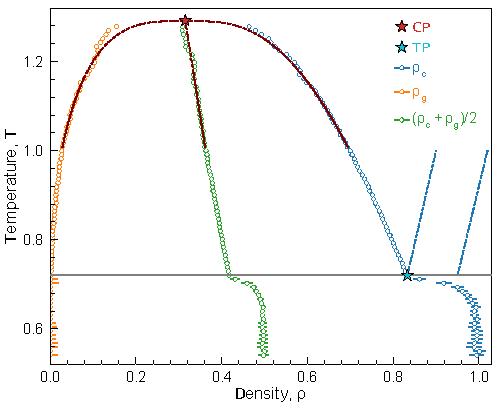
\includegraphics[width=\textwidth]{MACR-Figure-1.pdf}

        \end{figure}

      \end{column}

      \begin{column}{0.45\linewidth}

        \begin{equation}
          \rho_{c}-\rho_{g} \simeq A \tau^{\beta}, \quad \rho_{c}+\rho_{g} \simeq a \tau+2 \rho_{\mathrm{CP}},
          \label{eqFitFlatLayer}
        \end{equation}
        \jj{где $\tau=T_{\mathrm{CP}}-T$; \\
          $T_{\mathrm{CP}}$ и $\rho_{\mathrm{CP}}$ - температура и
          плотность в критической точке соответственно; \\
          $\beta$ - критический индекс.}

        \vspace{0.5cm}

        \jj $\beta = 0.5$ для LJ12-4 и $\beta = 0.325$ для других рассматриваемых потенциалов.

      \end{column}
    \end{columns}
  }

  \vspace{0.5cm}
  \tiny{E. Luijten et al., Physical Review Letters 89, 025703 (2002).\\
    F. Biscay, et al., The Journal of Physical Chemistry B 112, 13885 (2008).}
\end{frame}




\begin{frame}{Вычисление диффузии и спектров в жидкости}
  \footnotesize{
    \begin{columns}
      \begin{column}{0.5\linewidth}
        \begin{center}
          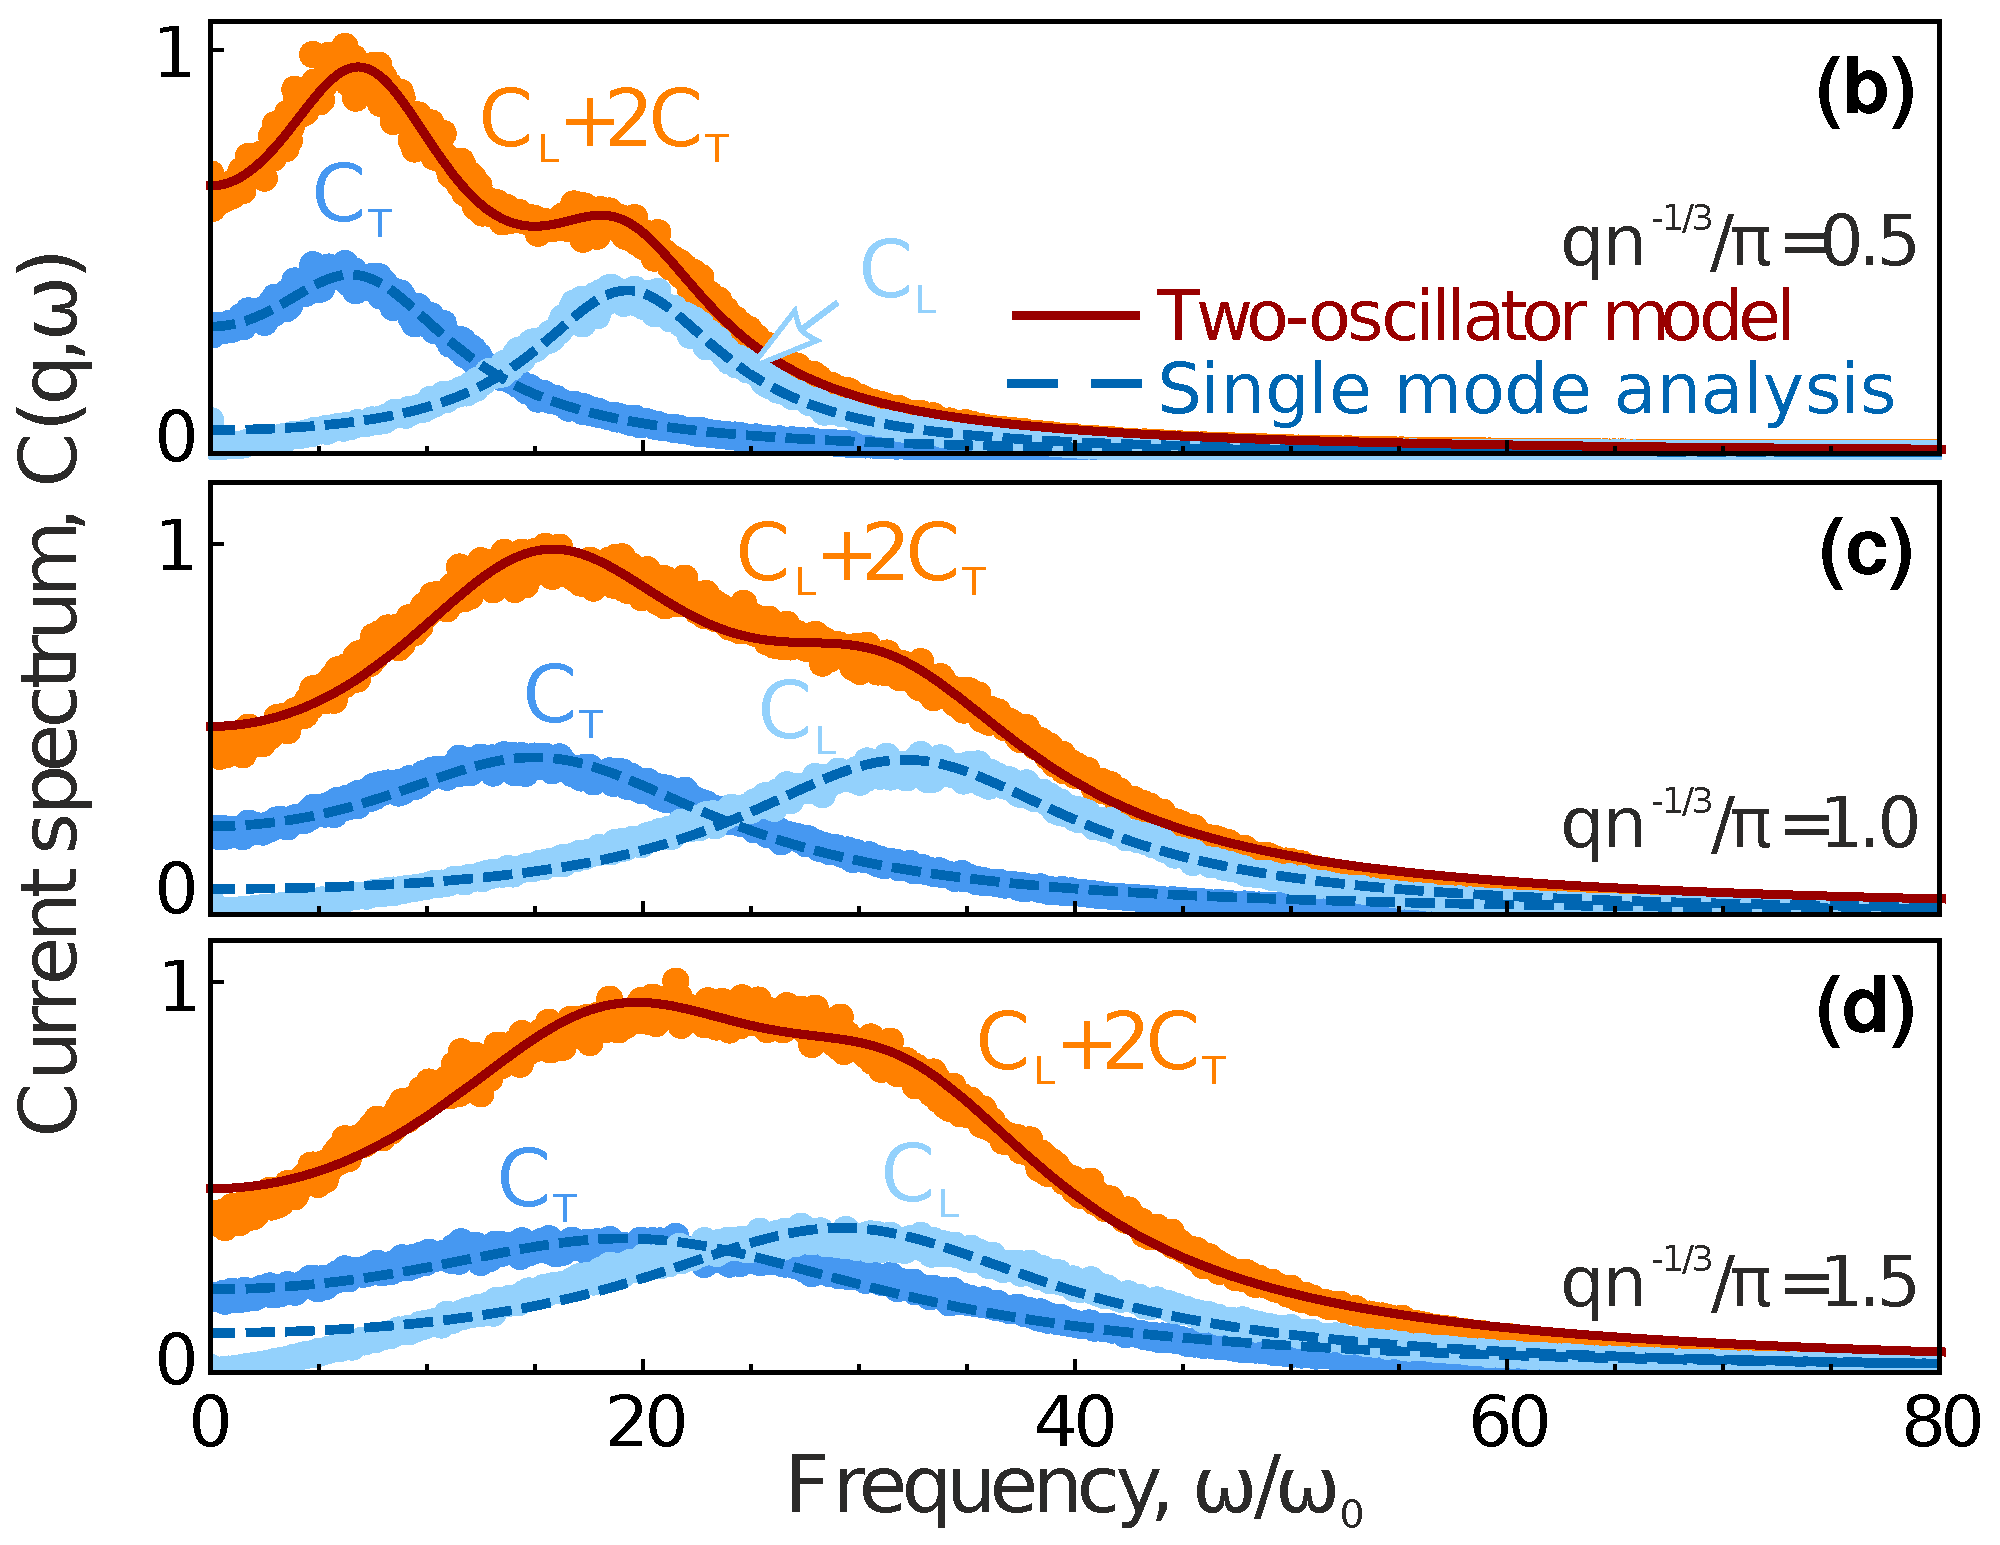
\includegraphics[width=\textwidth]{CFS-Figure1.png}
        \end{center}

      \end{column}

      \begin{column}{0.5\linewidth}

        Cреднеквадратичное смещение частиц:
        \begin{align}
          \sigma^2(t) &= \sum\limits_{\alpha = 1}^{N} (r_{\alpha}(t) - r_{\alpha}(0))^2 / N \\
          \sigma^2(t) &= 6\cdot D\cdot t
                        \label{eqRMS}
        \end{align}

        Подвижность частиц $\mu$ связана с диффузией:
        \begin{equation}
          \mu = \frac{D}{T}
          \label{eqMobility}
        \end{equation}

        Спектр потока скорости:
        \begin{align}
          C_{L, T}(\mathbf{q}, \omega)&=\int dt e^{i \omega t} \text{Re} \left\langle\mathbf{j}_{L, T}(\mathbf{q}, t) \mathbf{j}_{L, T}(-\mathbf{q}, 0)\right\rangle \\
          \text{где} \quad \mathbf{j}(\mathbf{q}, t)&=N^{-1} \sum_{s} \mathbf{v}_{s}(t) \exp \left(i \mathbf{q} \mathbf{r}_{s}(t)\right)
        \end{align}

      \end{column}
    \end{columns}

    \vspace{0.5cm}

    Полный спектр потока скорости $C(q, \omega) = C_L(q, \omega) + (D-1)C_T(q, \omega)$:
    \begin{equation}
      \begin{aligned}
        C(q, \omega) & \propto \frac{\Gamma_{L}}{\left(\omega-\omega_{L}\right)^{2}+\Gamma_{L}^{2}}+\frac{\Gamma_{L}}{\left(\omega+\omega_{L}\right)^{2}+\Gamma_{L}^{2}}+\frac{(D-1) \Gamma_{T}}{\left(\omega-\omega_{T}\right)^{2}+\Gamma_{T}^{2}}+\frac{(D-1) \Gamma_{T}}{\left(\omega+\omega_{T}\right)^{2}+\Gamma_{T}^{2}}
      \end{aligned}
      \label{eq5}
    \end{equation}
  }
  \vspace{1.0cm}
  \tiny{N.P. Kryuchkov, et al., Scientific Reports 9, 10483 (2019). \\
    S.A. Khrapak, et al., The Journal of Chemical Physics 149, 134114 (2018).}

\end{frame}




\begin{frame}{Результаты вычисления фазовых диаграмм и подвижности}
  \footnotesize{
    \begin{figure}
      \centering
      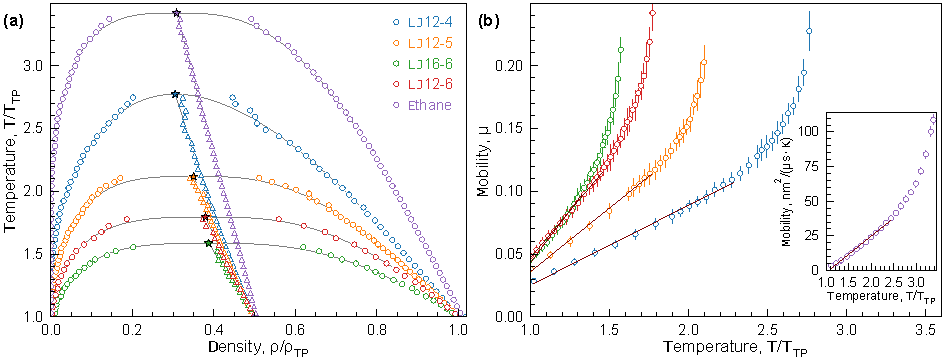
\includegraphics[width=\textwidth]{MACR-Figure3}
      \caption{\footnotesize{\textbf{(a) Фазовые диаграммы рассматриваемых потенциалов:} фазовые диаграммы рассчитанные плоским слоем.\\
          \textbf{(b) Температурная зависимость подвижности частиц:} подвижность частиц рассчитанная на бинодали жидкость -- газ.}}
    \end{figure}
  }

  \tiny{Influence of Long-Range Potential Action on Mobility on a Liquid Binodal / Nikita A. Dmitryuk, Lucia A. Mistryukova, Nikita P. Kryuchkov, Sergey A. Khrapak, Stanislav O. Yurchenko. // \textit{The Journal of Chemical Physics}}
\end{frame}




\begin{frame}{Результаты совместного анализа}
  \scriptsize{

    \begin{figure}
      \centering
      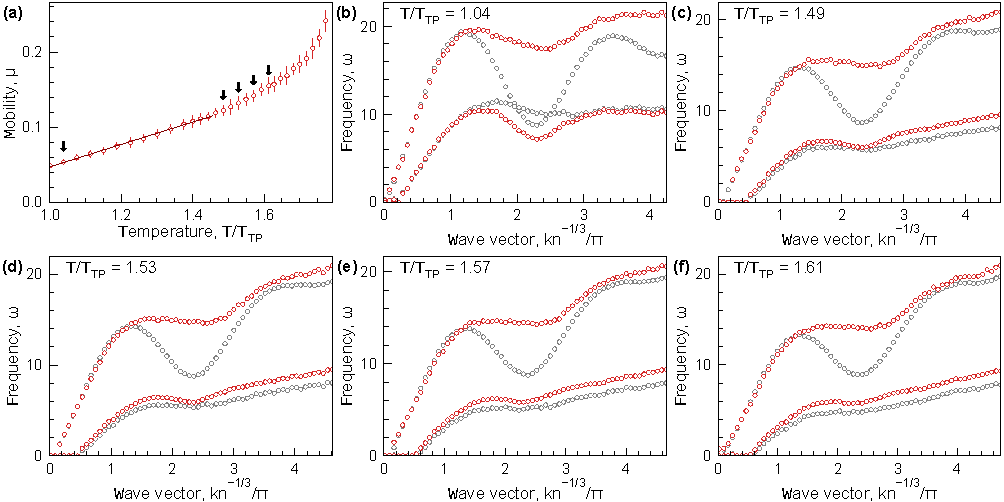
\includegraphics[width=0.95\textwidth]{MACR-Figure4}
      \caption{\scriptsize{\textbf{(a) Температурная зависимость подвижности потенциала LJ12-6:} точки, в который были рассчитаны спектры указаны черными стрелками.\\
          \textbf{(b) - (f) Спектры потенциала LJ12-6:} Красным цветом показаны спектры, рассчитанные совместным анализом мод.}}
      \label{Figure4}
    \end{figure}
  }

  \tiny{Influence of Long-Range Potential Action on Mobility on a Liquid Binodal / Nikita A. Dmitryuk, Lucia A. Mistryukova, Nikita P. Kryuchkov, Sergey A. Khrapak, Stanislav O. Yurchenko. // \textit{The Journal of Chemical Physics}}
\end{frame}




\begin{frame}{Тесты на устойчивость метода}
  \footnotesize{
    \begin{figure}[!t]
      \centering
      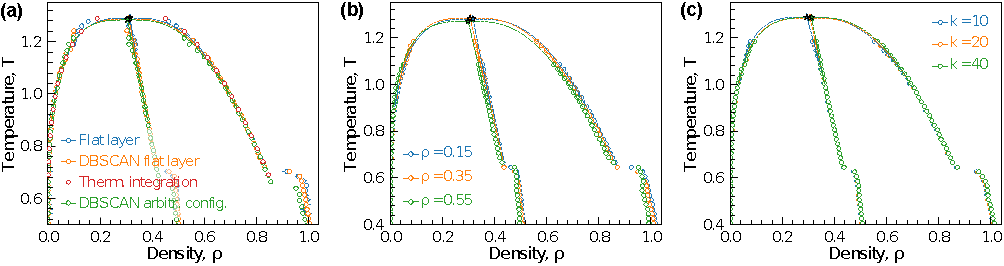
\includegraphics[width=\linewidth]{Figure10.pdf}
      \caption{\textbf{(a)} Сравнение различных методов построения фазовых диаграмм. Красным отмечен самый точный метод - термодинамическое интегрирование.\\
        \textbf{(b)} Тест на влияние средней плотности на фазовую диаграмму системы LJ12-6 в трехмерии.\\
        \textbf{(c)} Тест на влияние начального параметра $k$ на фазовую диаграмму системы LJ12-6 в трехмерии.}
      \label{tests}
    \end{figure}
  }

\end{frame}




\begin{frame}{Скорость нуклеации в переохлажденных системах}
  \footnotesize{

    \begin{figure}[!t]
      \centering
      \includegraphics[width=\linewidth]{otchet.pdf}
      \label{otchet}
    \end{figure}

    Процесс зарождения и роста кластеров в переохлажденной системе частиц.

    \begin{figure}[!t]
      \centering
      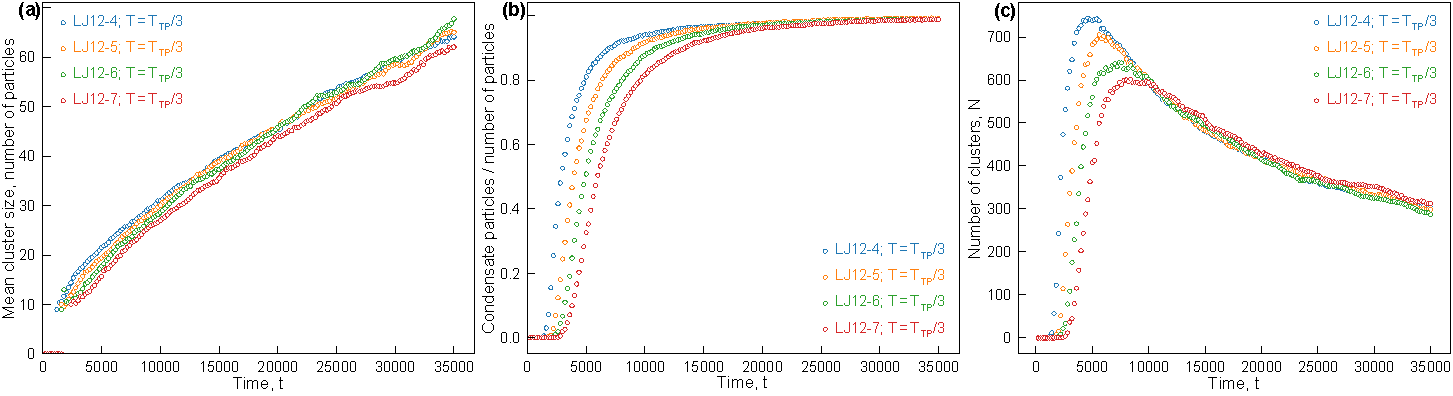
\includegraphics[width=\linewidth]{nucleation.pdf}
      \label{nucleation}
    \end{figure}
  }

\end{frame}




\begin{frame}{Заключение}
  \footnotesize{

    \textbf{Научная новизна:}

    \begin{itemize}

    \item Установлено, что подвижность имеет линейную температурную зависимость в широком диапазоне на бинодали жидкость-газ.

    \item При увеличении дальнодействия потенциала увеличивается отношение температур критической к тройной точке. Кроме того, при этом уменьшается наклон температурной зависимости подвижности.

    \item Отклонение подвижности от линейной зависимости при высоких температурах коррелирует с переходом спектров возбуждений от осцилирующего к монотонному виду.

    \end{itemize}

    \textbf{Новизна метода:}

    \begin{itemize}

    \item Разработан новый метода классификации частиц в двухфазных системах на основе алгоритма кластеризации DBSCAN. Алгоритм показывает высокую точность распознавания фаз, и открывает новые области для изучения, например влияние дальнодействия потенциала на скорость нуклеации в переохлажденных системах.

    \end{itemize}
  }
\end{frame}




\begin{frame}{Апробация}
  \footnotesize{

    \textbf{Публикации:}

    \begin{itemize}
    \item Kryuchkov, N. P., Dmitryuk, N. A., Li, W., Ovcharov, P. V., Han, Y., Sapelkin, A. V., and Yurchenko, S. O. (2021). Mean-field model of melting in superheated crystals based on a single experimentally measurable order parameter. Scientific reports, 11(1), 1-15.
    \item Yakovlev, E. V., Kryuchkov, N. P., Korsakova, S. A., Dmitryuk, N. A., Ovcharov, P. V., Andronic, M. M., ... and Yurchenko, S. O. (2022). 2D colloids in rotating electric fields: A laboratory of strong tunable three-body interactions. Journal of Colloid and Interface Science, 608, 564-574.
    \item Tsiok, E. N., Fomin, Y. D., Gaiduk, E. A., Tareyeva, E. E., Ryzhov, V. N., Libet, P. A., ... Yurchenko, S. O. (2022). The role of attraction in the phase diagrams and melting scenarios of generalized 2D Lennard-Jones systems. The Journal of Chemical Physics, 156(11), 114703.
    \end{itemize}

    \textbf {Результаты работ представлены на следующих конференциях:}

    \begin{itemize}
    \item XX Школа-конференция молодых ученых <<Проблемы физики твердого тела и высоких давлений>>, Сочи, 16-26 сентября 2021г.
    \item Современные тенденции развития функциональных материалов, Сочи, 11-14 ноября 2021г.
    \item Dynamic phenomena workshop 2022.
    \end{itemize}
  }
\end{frame}




\begin{frame}{Используемые технологии}

  \begin{columns}
    \begin{column}{0.3\linewidth}
      \begin{center}
        
\includegraphics[width=\textwidth]{git_logo.png}
        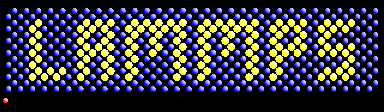
\includegraphics[width=\textwidth]{lammps_logo.png}
        
\includegraphics[width=\textwidth]{latex_logo.png}
        
\includegraphics[width=\textwidth]{docker_logo.png}
      \end{center}
    \end{column}

    \begin{column}{0.3\linewidth}
      \begin{center}
        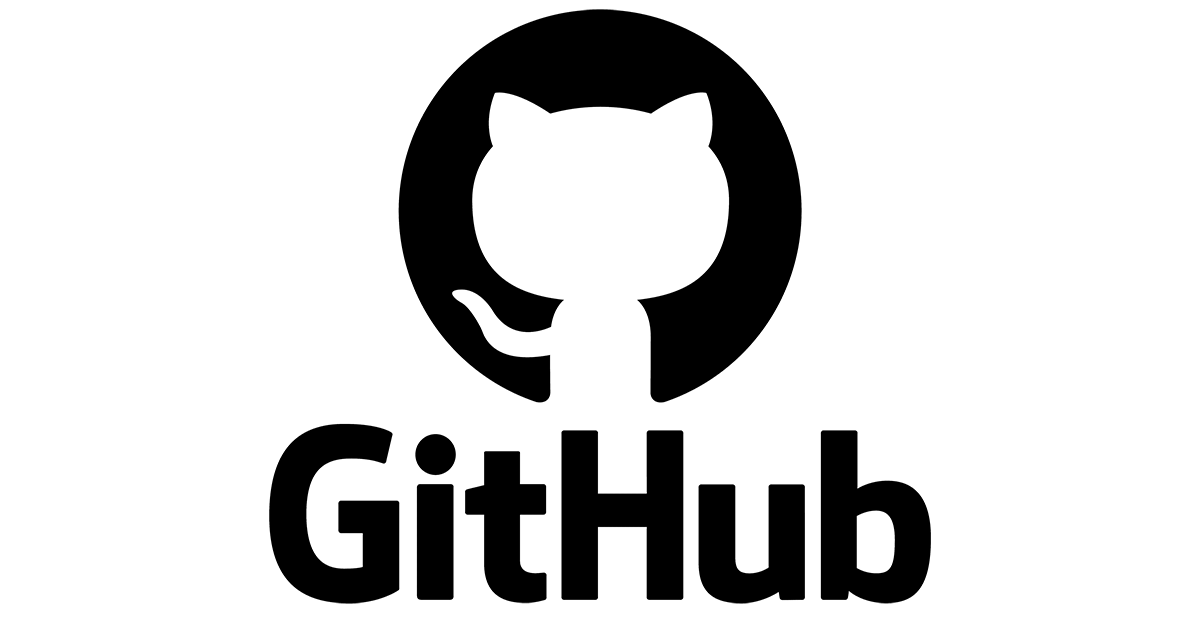
\includegraphics[width=\textwidth]{github_logo.png}
        
\includegraphics[width=\textwidth]{povray_logo.png}
        
\includegraphics[width=\textwidth]{matlab_logo.png}
      \end{center}
    \end{column}

    \begin{column}{0.3\linewidth}
      \begin{center}
        
\includegraphics[width=\textwidth]{jenkins_logo.png}
        
\includegraphics[width=\textwidth]{linux_logo.png}
        
\includegraphics[width=\textwidth]{python_logo.png}
      \end{center}
    \end{column}
  \end{columns}
\end{frame}




\begin{frame}
  \centering \Huge \textcolor{blue}{Ваши вопросы!}
\end{frame}




\begin{frame}{Результаты совместного анализа}
  \footnotesize{

    \begin{figure}
      \centering
      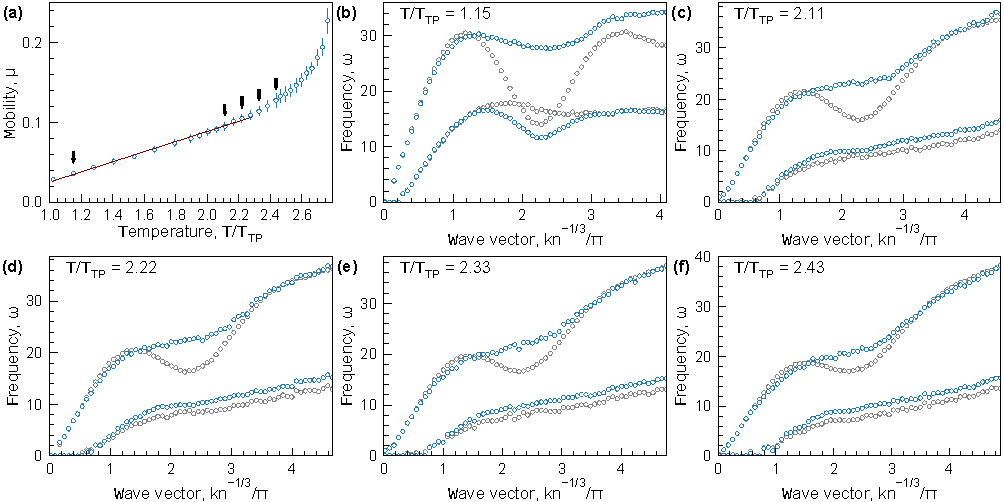
\includegraphics[width=\textwidth]{MACR-Figure5}
      \caption{\footnotesize \textbf{Аналогичные графики для потенциала LJ12-4}}
      \label{Figure4}
    \end{figure}

  }

  \tiny{Influence of Long-Range Potential Action on Mobility on a Liquid Binodal / Nikita A. Dmitryuk, Lucia A. Mistryukova, Nikita P. Kryuchkov, Sergey A. Khrapak, Stanislav O. Yurchenko. // \textit{The Journal of Chemical Physics}}
\end{frame}




\begin{frame}{Результаты совместного анализа}
  \footnotesize{

    \begin{figure}
      \centering
      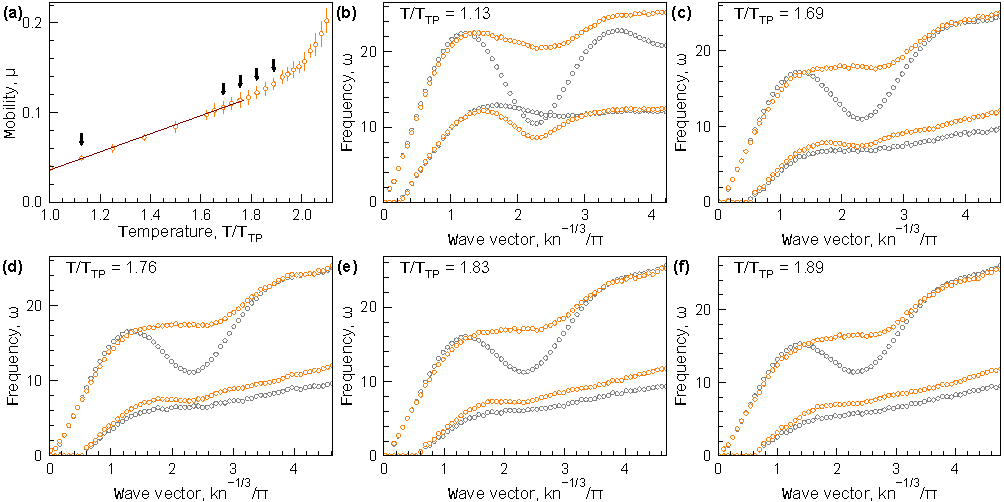
\includegraphics[width=\textwidth]{MACR-Figure6}
      \caption{\footnotesize \textbf{Аналогичные графики для потенциала LJ12-5}}
      \label{Figure4}
    \end{figure}

  }

  \tiny{Influence of Long-Range Potential Action on Mobility on a Liquid Binodal / Nikita A. Dmitryuk, Lucia A. Mistryukova, Nikita P. Kryuchkov, Sergey A. Khrapak, Stanislav O. Yurchenko. // \textit{The Journal of Chemical Physics}}
\end{frame}




\begin{frame}{Результаты совместного анализа}
  \footnotesize{

    \begin{figure}
      \centering
      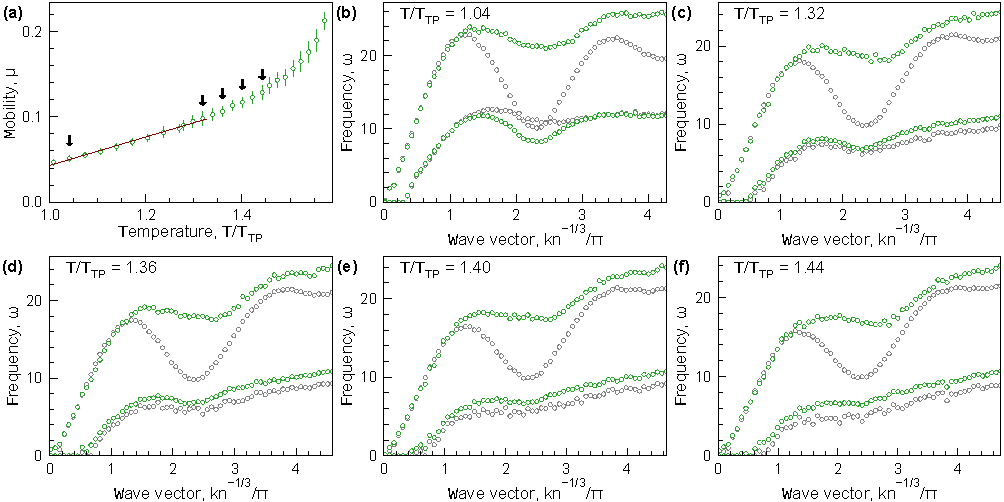
\includegraphics[width=\textwidth]{MACR-Figure7}
      \caption{\footnotesize \textbf{Аналогичные графики для потенциала LJ16-6}}
      \label{Figure4}
    \end{figure}
  }

  \tiny{Influence of Long-Range Potential Action on Mobility on a Liquid Binodal / Nikita A. Dmitryuk, Lucia A. Mistryukova, Nikita P. Kryuchkov, Sergey A. Khrapak, Stanislav O. Yurchenko. // \textit{The Journal of Chemical Physics}}
\end{frame}




\begin{frame}{Зависимость положения тройных и критических точек}
  \footnotesize{

    \begin{figure}
      \centering
      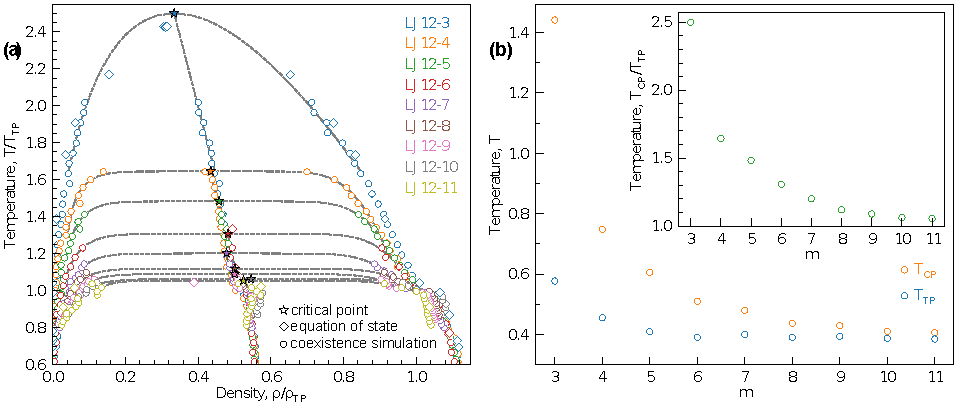
\includegraphics[width=\textwidth]{NMP-Figure4}
      \caption{\footnotesize \textbf{Зависимость тройных и критических точек от дальнодействия притяжения в системе}}
      \label{Figure4}
    \end{figure}
  }

  \tiny{Tsiok, E. N., Dmitryuk, N.A, ... Yurchenko, S. O. (2022). The role of attraction in the phase diagrams and melting scenarios of generalized 2D Lennard-Jones systems. // \textit{The Journal of Chemical Physics}}
\end{frame}




\end{document}
